% Options for packages loaded elsewhere
\PassOptionsToPackage{unicode}{hyperref}
\PassOptionsToPackage{hyphens}{url}
%
\documentclass[
]{book}
\usepackage{lmodern}
\usepackage{amssymb,amsmath}
\usepackage{ifxetex,ifluatex}
\ifnum 0\ifxetex 1\fi\ifluatex 1\fi=0 % if pdftex
  \usepackage[T1]{fontenc}
  \usepackage[utf8]{inputenc}
  \usepackage{textcomp} % provide euro and other symbols
\else % if luatex or xetex
  \usepackage{unicode-math}
  \defaultfontfeatures{Scale=MatchLowercase}
  \defaultfontfeatures[\rmfamily]{Ligatures=TeX,Scale=1}
\fi
% Use upquote if available, for straight quotes in verbatim environments
\IfFileExists{upquote.sty}{\usepackage{upquote}}{}
\IfFileExists{microtype.sty}{% use microtype if available
  \usepackage[]{microtype}
  \UseMicrotypeSet[protrusion]{basicmath} % disable protrusion for tt fonts
}{}
\makeatletter
\@ifundefined{KOMAClassName}{% if non-KOMA class
  \IfFileExists{parskip.sty}{%
    \usepackage{parskip}
  }{% else
    \setlength{\parindent}{0pt}
    \setlength{\parskip}{6pt plus 2pt minus 1pt}}
}{% if KOMA class
  \KOMAoptions{parskip=half}}
\makeatother
\usepackage{xcolor}
\IfFileExists{xurl.sty}{\usepackage{xurl}}{} % add URL line breaks if available
\IfFileExists{bookmark.sty}{\usepackage{bookmark}}{\usepackage{hyperref}}
\hypersetup{
  pdftitle={R Ders Notları},
  pdfauthor={Dr.~Busenur Kızılaslan},
  hidelinks,
  pdfcreator={LaTeX via pandoc}}
\urlstyle{same} % disable monospaced font for URLs
\usepackage{color}
\usepackage{fancyvrb}
\newcommand{\VerbBar}{|}
\newcommand{\VERB}{\Verb[commandchars=\\\{\}]}
\DefineVerbatimEnvironment{Highlighting}{Verbatim}{commandchars=\\\{\}}
% Add ',fontsize=\small' for more characters per line
\usepackage{framed}
\definecolor{shadecolor}{RGB}{248,248,248}
\newenvironment{Shaded}{\begin{snugshade}}{\end{snugshade}}
\newcommand{\AlertTok}[1]{\textcolor[rgb]{0.94,0.16,0.16}{#1}}
\newcommand{\AnnotationTok}[1]{\textcolor[rgb]{0.56,0.35,0.01}{\textbf{\textit{#1}}}}
\newcommand{\AttributeTok}[1]{\textcolor[rgb]{0.77,0.63,0.00}{#1}}
\newcommand{\BaseNTok}[1]{\textcolor[rgb]{0.00,0.00,0.81}{#1}}
\newcommand{\BuiltInTok}[1]{#1}
\newcommand{\CharTok}[1]{\textcolor[rgb]{0.31,0.60,0.02}{#1}}
\newcommand{\CommentTok}[1]{\textcolor[rgb]{0.56,0.35,0.01}{\textit{#1}}}
\newcommand{\CommentVarTok}[1]{\textcolor[rgb]{0.56,0.35,0.01}{\textbf{\textit{#1}}}}
\newcommand{\ConstantTok}[1]{\textcolor[rgb]{0.00,0.00,0.00}{#1}}
\newcommand{\ControlFlowTok}[1]{\textcolor[rgb]{0.13,0.29,0.53}{\textbf{#1}}}
\newcommand{\DataTypeTok}[1]{\textcolor[rgb]{0.13,0.29,0.53}{#1}}
\newcommand{\DecValTok}[1]{\textcolor[rgb]{0.00,0.00,0.81}{#1}}
\newcommand{\DocumentationTok}[1]{\textcolor[rgb]{0.56,0.35,0.01}{\textbf{\textit{#1}}}}
\newcommand{\ErrorTok}[1]{\textcolor[rgb]{0.64,0.00,0.00}{\textbf{#1}}}
\newcommand{\ExtensionTok}[1]{#1}
\newcommand{\FloatTok}[1]{\textcolor[rgb]{0.00,0.00,0.81}{#1}}
\newcommand{\FunctionTok}[1]{\textcolor[rgb]{0.00,0.00,0.00}{#1}}
\newcommand{\ImportTok}[1]{#1}
\newcommand{\InformationTok}[1]{\textcolor[rgb]{0.56,0.35,0.01}{\textbf{\textit{#1}}}}
\newcommand{\KeywordTok}[1]{\textcolor[rgb]{0.13,0.29,0.53}{\textbf{#1}}}
\newcommand{\NormalTok}[1]{#1}
\newcommand{\OperatorTok}[1]{\textcolor[rgb]{0.81,0.36,0.00}{\textbf{#1}}}
\newcommand{\OtherTok}[1]{\textcolor[rgb]{0.56,0.35,0.01}{#1}}
\newcommand{\PreprocessorTok}[1]{\textcolor[rgb]{0.56,0.35,0.01}{\textit{#1}}}
\newcommand{\RegionMarkerTok}[1]{#1}
\newcommand{\SpecialCharTok}[1]{\textcolor[rgb]{0.00,0.00,0.00}{#1}}
\newcommand{\SpecialStringTok}[1]{\textcolor[rgb]{0.31,0.60,0.02}{#1}}
\newcommand{\StringTok}[1]{\textcolor[rgb]{0.31,0.60,0.02}{#1}}
\newcommand{\VariableTok}[1]{\textcolor[rgb]{0.00,0.00,0.00}{#1}}
\newcommand{\VerbatimStringTok}[1]{\textcolor[rgb]{0.31,0.60,0.02}{#1}}
\newcommand{\WarningTok}[1]{\textcolor[rgb]{0.56,0.35,0.01}{\textbf{\textit{#1}}}}
\usepackage{longtable,booktabs}
% Correct order of tables after \paragraph or \subparagraph
\usepackage{etoolbox}
\makeatletter
\patchcmd\longtable{\par}{\if@noskipsec\mbox{}\fi\par}{}{}
\makeatother
% Allow footnotes in longtable head/foot
\IfFileExists{footnotehyper.sty}{\usepackage{footnotehyper}}{\usepackage{footnote}}
\makesavenoteenv{longtable}
\usepackage{graphicx,grffile}
\makeatletter
\def\maxwidth{\ifdim\Gin@nat@width>\linewidth\linewidth\else\Gin@nat@width\fi}
\def\maxheight{\ifdim\Gin@nat@height>\textheight\textheight\else\Gin@nat@height\fi}
\makeatother
% Scale images if necessary, so that they will not overflow the page
% margins by default, and it is still possible to overwrite the defaults
% using explicit options in \includegraphics[width, height, ...]{}
\setkeys{Gin}{width=\maxwidth,height=\maxheight,keepaspectratio}
% Set default figure placement to htbp
\makeatletter
\def\fps@figure{htbp}
\makeatother
\usepackage[normalem]{ulem}
% Avoid problems with \sout in headers with hyperref
\pdfstringdefDisableCommands{\renewcommand{\sout}{}}
\setlength{\emergencystretch}{3em} % prevent overfull lines
\providecommand{\tightlist}{%
  \setlength{\itemsep}{0pt}\setlength{\parskip}{0pt}}
\setcounter{secnumdepth}{5}
\usepackage{booktabs}
\usepackage[]{natbib}
\bibliographystyle{apalike}

\title{R Ders Notları}
\author{Dr.~Busenur Kızılaslan}
\date{2020-10-13}

\begin{document}
\maketitle

{
\setcounter{tocdepth}{1}
\tableofcontents
}
\hypertarget{uxf6n-bilgi}{%
\chapter{Ön Bilgi}\label{uxf6n-bilgi}}

R ders notları temelde \emph{BSP2043 - Bilgisayar III} ve \emph{BSP2044 - Bilgisayar IV} derslerine kaynaklık etmesi amacıyla tasarlanmış olup konu çerçevesinde kendisini geliştirmek isteyen herkesin faydalanabilmesi hedeflenmiştir.

Kaynak, temel matematik ve ingilizce bilgisine sahip olan herkesin anlayıp uygulayabileceği basitlikte bir anlatıma sahiptir.

Ders dili Türkçe'dir. Bu bakımdan genel anlatımda Türkçe kullanılacaktır. Literatürü rahat takip edebilmeniz, komut karmaşası yaşamamanız ve araştırma sürecinde zengin forum imkanından yararlanabilmeniz adına temel terimler orijinal haliyle kullanılacaktır.

Aynı zamanda referans verilen kaynaklar da orijinal dili ile paylaşılacaktır. Bu nedenle İngilizce eksikliğinizi gidermeniz önerilir.

Kaynaklar;

\begin{itemize}
\tightlist
\item
  Kitaplar
\end{itemize}

\href{https://www.cs.upc.edu/~robert/teaching/estadistica/TheRBook.pdf}{The R Book - Michael J. Crawley}

\href{https://r4ds.had.co.nz}{R for Data Science - Hadley Wickham, Garrett Grolemund}

\href{https://rafalab.github.io/dsbook/}{Introduction to Data Science - Rafael A. Irizarry}

\href{https://bookdown.org/rdpeng/rprogdatascience/}{R Programming for Data Science - Roger D. Peng}

\href{https://web.itu.edu.tr/~tokerem/The_Book_of_R.pdf}{The Book of R - Tilman M. Davies}

\begin{itemize}
\tightlist
\item
  Eğitimler
\end{itemize}

\href{https://www.edx.org/course/data-science-r-basics}{HarvardX - Data Science: R Basics}

\href{https://www.edx.org/course/data-science-visualization}{HarvardX - Data Science: Visualization}

\href{https://www.edx.org/course/data-science-probability}{HarvardX - Data Science: Probability}

Katkı ve öneriler için: \texttt{busenur.sarica@marmara.edu.tr}

İyi eğlenceler!

\hypertarget{hakkux131mda}{%
\section{Hakkımda}\label{hakkux131mda}}

2012 yılında Mimar Sinan G. S. Üniversitesi istatistik bölümünde lisans öğrenimimi tamamlamamın ardından 2014 yılı itibariyle Marmara Üniversitesi istatistik bölümünde araştırma görevlisi olarak göreve başladım. Eş zamanlı olarak başladığım yüksek lisans öğrenimimi yine Mimar Sinan G. S. Üniversitesi istatistik anabilim dalında tamamlarken artık çalışma alanım bulanık mantık (\href{https://en.wikipedia.org/wiki/Fuzzy_logic}{fuzzy logic}) olarak şekillenmişti. Bir buçuk yılda tamamladığım yüksek lisansın ardından farklı bakış açısı kazanma fikriyle yönümü Yıldız Teknik Üniversitesi'ne çevirdim. 2015 yılında istatistik bölümünde başladığım doktora öğrenimimi 2020 yılında yine bulanık mantık ile öngörü üzerine hazırladığım tezim ile tamamladım. Doktora öğrenimim sırasında İstanbul Teknik Üniversitesi endüstri mühendisliği bölümünden de çeşitli dersler alarak alanında uzman hocaların\footnote{\href{http://akademi.itu.edu.tr/kahramanc/}{Prof.~Dr.~Cengiz Kahraman}} bilgilerinden faydalanma imkanı buldum.

Akademik kariyer hedefiyle başlamadığım öğrenim yaşamımda ufku açık, aydınlık ve birikimli hocalarım yolumu bulmama yardımcı olmuştur. 2018 yılında Polonya'da gerçekleşen \href{http://www.linstat2018.put.poznan.pl/ysa.html}{International Conference on Trends and Perspectives in Linear Statistical Inference (LinStat'2018)} kapsamında sunduğum, doktora tezimin bir kısmından oluşan çalışma ile aldığım Young Scientists Awards ikincilik ödülü de yanlış yolda olmadığımı göstermiştir.

Üzerimde emeği olan herkese teşekkürlerimle!

\href{https://avesis.marmara.edu.tr/busenur.sarica}{\textbf{CV}}, \href{https://scholar.google.com.tr/citations?user=OKlYJEgAAAAJ\&hl=tr}{\textbf{Google Scholar}}, \href{https://www.linkedin.com/in/busenur-kızılaslan-795ab54a}{\textbf{Linkedin}}

\hypertarget{motivasyon}{%
\chapter{Motivasyon}\label{motivasyon}}

\textbf{`Bu dersi neden alıyorum?'} sorusuna karşılık olarak alacağınız cevap \textbf{`ilerleyen dönemlerde göreceğiniz derslerin uygulamalarında ihtiyaç duyacaksınız'}dan çok daha fazlası! Herhangi bir programlama diline hakim olmak veriyi anlamlandırabilmek adına zaten önemliyken özellikle R, Python gibi açık kaynak ve hızla gelişmeye devam eden programlama dillerini biliyor olmak sizleri donanımlı kılacaktır.


\includegraphics[width=0.85\textwidth,height=\textheight]{/Users/busenursarica/Desktop/R Lec Notes/comp3/_book/comp3_files/figure-html/steve.png}

Programlama bilgisine sahip olmak iş yaşamındaki ihtiyacınızı karşılamasının yanı sıra günlük yaşamdaki problem çözme yeteneğinizin gelişmesine de yardımcı olmaktadır. Programlama yapısını öğrenen kişinin diğer programlama dillerini öğrenmesi kolaylaşmaktadır. İş başvurularında birden fazla programlama dili biliyor olmanın sizi öne çıkaracağı da aşikar. Burada sorulması gereken asıl soru \textbf{`hangi programlama dilini/dillerini öğrenmeliyim?'} olmalıdır. Ders kapsamında R programlama dili ve özellikleri açıklanacaktır.


\includegraphics[width=0.85\textwidth,height=\textheight]{/Users/busenursarica/Desktop/R Lec Notes/comp3/_book/comp3_files/figure-html/bill.png}

\hypertarget{genel-bakux131ux15f}{%
\chapter{Genel Bakış}\label{genel-bakux131ux15f}}

\hypertarget{r-nedir}{%
\section{R: Nedir?}\label{r-nedir}}

İstatistiksel analiz ve veri görselleştirme amacıyla geliştirilen R, açık kaynak olup ücretsizdir. R, dizayn olarak var olan iki dilden etkilenmiştir; Becker, Chambers \& Wilks'in S programlama dili ve Sussman'ın Scheme programlama dilidir. R, başlangıçta Yeni Zelanda Auckland'daki Auckland Üniversitesi İstatistik Bölümü'nde Ross Ihaka ve Robert Gentleman tarafından yazılmıştır. Ek olarak, büyük bir grup insan, kod ve hata raporları göndererek katkıda bulunmuştur. Tarihçeyi merak edenler \emph{A Brief History of S} \citep{Becker2004} kaynağını inceleyebilir.

1997 ortalarından itibaren çekirdek bir yapı \emph{(The R Core Team)} yönetimi sürdürmektedir.

\href{http://www.r-project.org}{Resmi internet adresi}

\href{http://www.cran.r-project.org}{Yükleme adresi}

\href{https://journal.r-project.org}{The R Journal}: R kullanıcıları için hakemli ve açık erişimli dergi

\href{https://www.r-project.org/doc/bib/R-books.html}{Kitaplar}: R kullancıları için çeşitli alanlarda/dillerde kaynak kitaplar

\href{http://www.statmethods.net}{Faydalı adres1}

\href{https://stackoverflow.com/questions/tagged/r}{Faydalı adres2}

\begin{verbatim}
Hangi komutun ne işe yaradığını anımsayamıyorsanız veya bir hata ile karşılaştıysanız
GOOGLE kullanın.
\end{verbatim}

\begin{verbatim}
Programlama öğrenmenin en iyi yolu denemek ve hata yapmaktır.
\end{verbatim}

\begin{center}\rule{0.5\linewidth}{0.5pt}\end{center}

\hypertarget{rstudio}{%
\subsection{RStudio}\label{rstudio}}

R üzerinde doğrudan çalışabilir veya bir grafik ara yüzü olan RStudio'nun zengin özelliklerinden faydalanma imkanından yararlanabilirsiniz. Uygulama kolaylığı sağlayan bir entegre geliştirme ortamı \emph{(integrated development environment (IDE))} olan RStudio, Windows, Mac ve Linux ile çalışabilir. RStudio'yu kullanışlı kılan birçok özellik mevcuttur, bunlardan birkaçı şu şekilde sıralanabilir.

\begin{itemize}
\item
  Script
\item
  Kodlama geçmişi, güçlü grafiksel altyapı
\item
  Cheatsheetler
\item
  Değişken ve fonksiyon tamamlama özelliği
\end{itemize}

\begin{center}\rule{0.5\linewidth}{0.5pt}\end{center}

\hypertarget{r-neden}{%
\section{R: Neden?}\label{r-neden}}

Veri analizi için kullanılabilecek SAS, SPSS, Excel, MATLAB gibi birçok yazılım mevcutken neden R kullanıyoruz?

\begin{itemize}
\item
  Ücretsiz (open source)
\item
  Geniş kullanım kitlesi

  \begin{itemize}
  \item
    Dünyada 2 milyondan fazla kullanıcıya sahip
  \item
    Sürekli gelişmeye devam eden yapısı
  \item
    Geniş forum ağı
  \end{itemize}
\item
  Uygulama ve kullanım kolaylığı
\item
  Grafik ve görsel üretimindeki başarısı
\item
  Paket kullanım imkanı
\item
  Raporlama kolaylığı ve RMarkdown sayesinde kolay sunum
\end{itemize}

R aynı zamanda bazı dezavantajlara da sahiptir.

\begin{itemize}
\item
  Güncelleneme gereksinimi
\item
  Uzmanlaşmanın diğer programlara göre biraz daha zor olması
\end{itemize}

\begin{center}\rule{0.5\linewidth}{0.5pt}\end{center}

\hypertarget{r-help}{%
\section{R: Help}\label{r-help}}

R'da karşılacağınız problemler için menüde yer alan \texttt{Help} kısmını kullanabilir veya \href{https://stackoverflow.com/questions/tagged/r}{Stackoverflow} gibi forumlardan faydalanabilirsiniz. Windows, Mac işletim sistemleri ve genel sorular için üç farklı \href{https://cran.r-project.org/faqs.html}{FAQ (Frequently Asked Questions)} kısmı mevcuttur.

Kullanacağınız fonksiyonun ismini biliyorsanız \texttt{?} kullanarak yine help içeriğinden faydalanabilirsiniz.

\begin{Shaded}
\begin{Highlighting}[]
\NormalTok{?sum}
\end{Highlighting}
\end{Shaded}

Kullanacağınız fonksiyonun ismini biliyor fakat hangi pakette yer aldığını bilmiyorsanız bu noktada \texttt{find} komutu size yardımcı olacaktır.

\begin{Shaded}
\begin{Highlighting}[]
\KeywordTok{find}\NormalTok{(}\StringTok{"sum"}\NormalTok{)}
\end{Highlighting}
\end{Shaded}

\begin{verbatim}
## [1] "package:base"
\end{verbatim}

Kullanacağınız fonksiyon ile ilgili örnek araştırmak isterseniz \texttt{example} komutu işinizi görecektir.

\begin{Shaded}
\begin{Highlighting}[]
\KeywordTok{example}\NormalTok{(sum)}
\end{Highlighting}
\end{Shaded}

\begin{verbatim}
## 
## sum> ## Pass a vector to sum, and it will add the elements together.
## sum> sum(1:5)
## [1] 15
## 
## sum> ## Pass several numbers to sum, and it also adds the elements.
## sum> sum(1, 2, 3, 4, 5)
## [1] 15
## 
## sum> ## In fact, you can pass vectors into several arguments, and everything gets added.
## sum> sum(1:2, 3:5)
## [1] 15
## 
## sum> ## If there are missing values, the sum is unknown, i.e., also missing, ....
## sum> sum(1:5, NA)
## [1] NA
## 
## sum> ## ... unless  we exclude missing values explicitly:
## sum> sum(1:5, NA, na.rm = TRUE)
## [1] 15
\end{verbatim}

\begin{center}\rule{0.5\linewidth}{0.5pt}\end{center}

\hypertarget{paketler}{%
\section{Paketler}\label{paketler}}

R programlama dili ile kendi döngülerinizi oluşturabilir, özgün kodlarınızı yazabilirsiniz, aynı zamanda paketler yardımı ile yazılmış olan zengin hazır kod içeriğinden de faydalanabilirsiniz. Bu zengin içeriğe hazırladığınız paketler ile dahil olma imkanınız da mevcut.

\begin{verbatim}
Paket indirme konusunda problem yaşıyorsanız R'ı yönetici olarak çalıştırmayı deneyin. 
\end{verbatim}

\begin{verbatim}
Paket yükleme işleminin hızlı olabilmesi için size en yakın mirror seçimini yapmalısınız.
\end{verbatim}

\begin{quote}
Paketler kullanım kolaylığı ve zamandan kazanç sağlamakla birlikte kullanılmadan önce içeriğin dikkatlice incelenmesi önemlidir. Tanımlamaları iyi anlaşılmadan kullanılan paketlerle yanlış sonuçlar elde edilmesi kaçınılmazdır.
\end{quote}

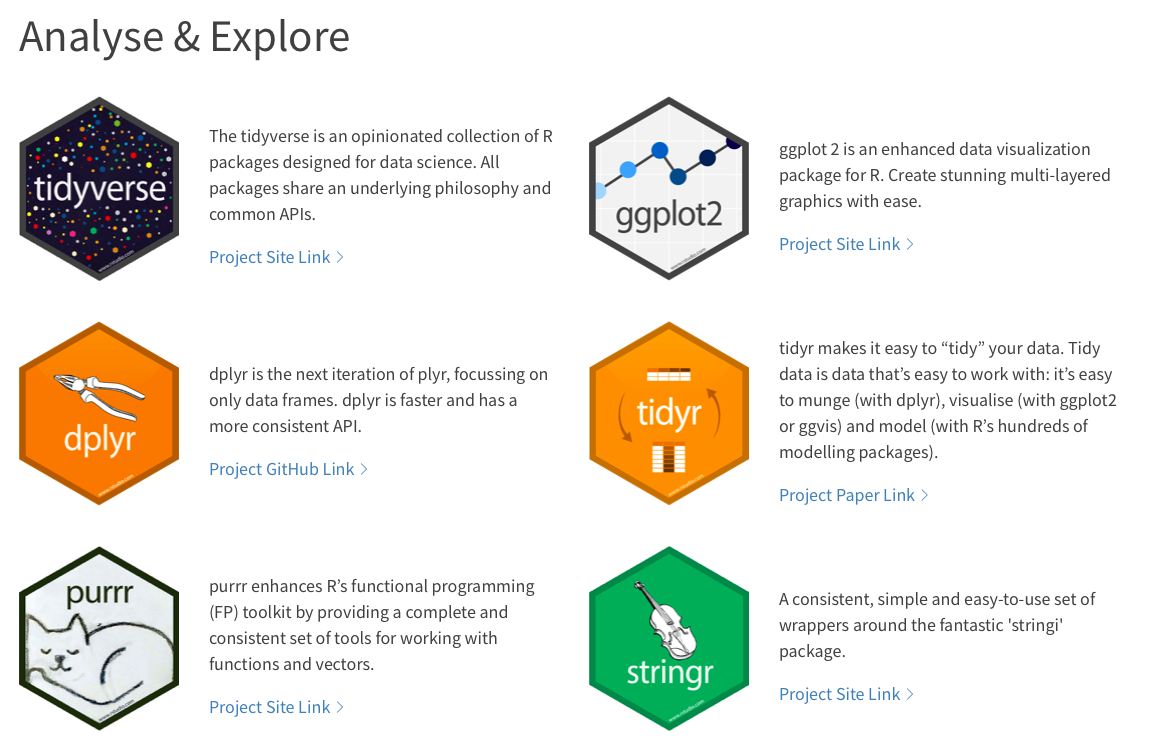
\includegraphics[width=0.85\textwidth,height=\textheight]{/Users/busenursarica/Desktop/R Lec Notes/comp3/_book/comp3_files/figure-html/P1.png}

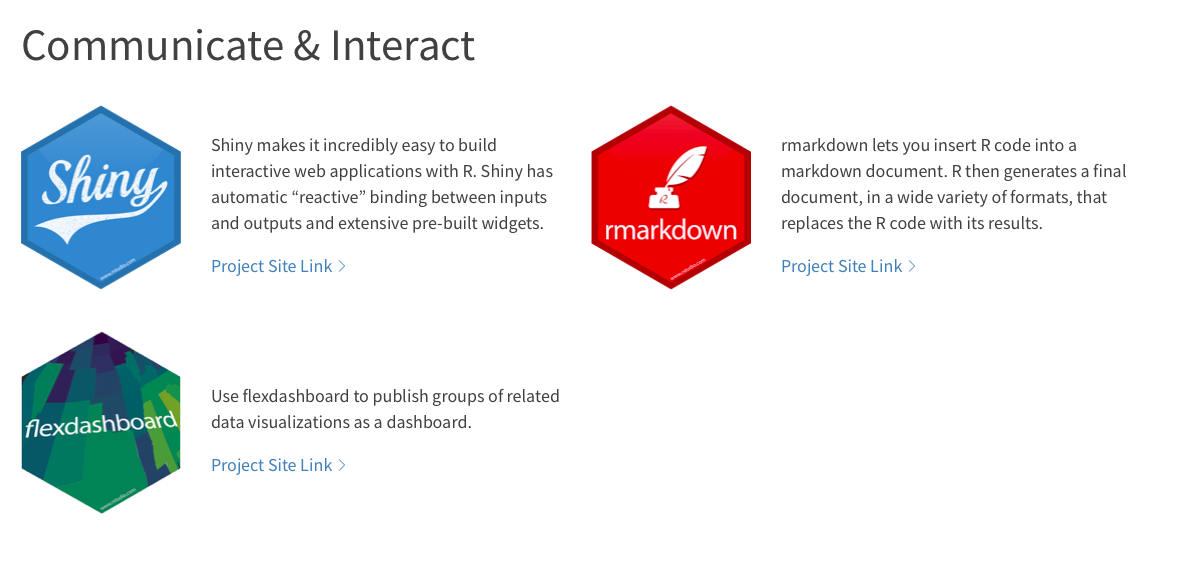
\includegraphics[width=0.85\textwidth,height=\textheight]{/Users/busenursarica/Desktop/R Lec Notes/comp3/_book/comp3_files/figure-html/P2.png}

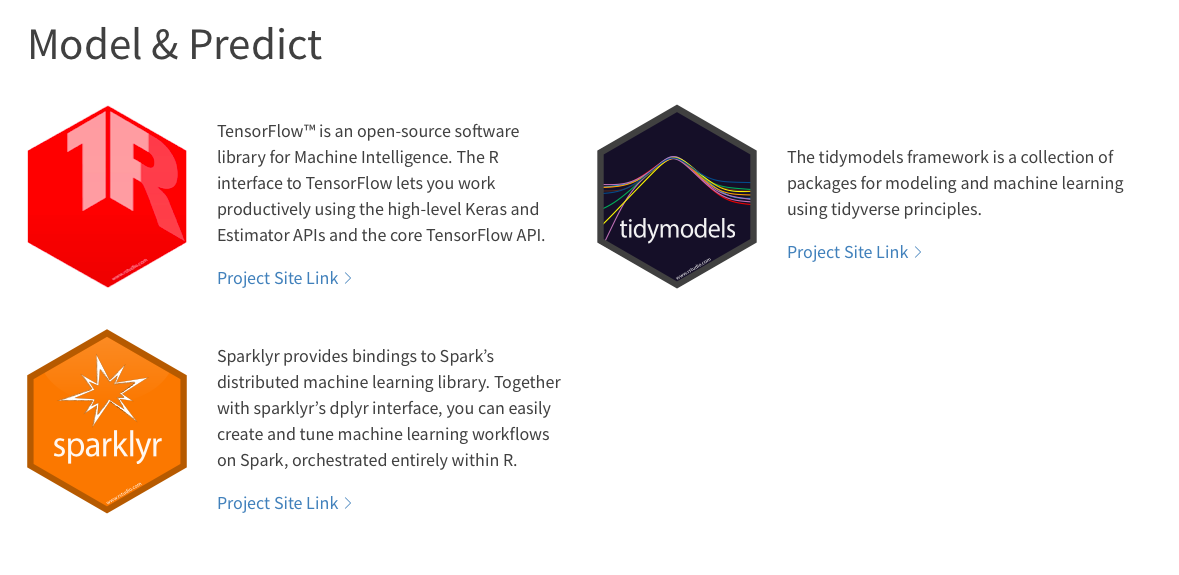
\includegraphics[width=0.85\textwidth,height=\textheight]{/Users/busenursarica/Desktop/R Lec Notes/comp3/_book/comp3_files/figure-html/P3.png}

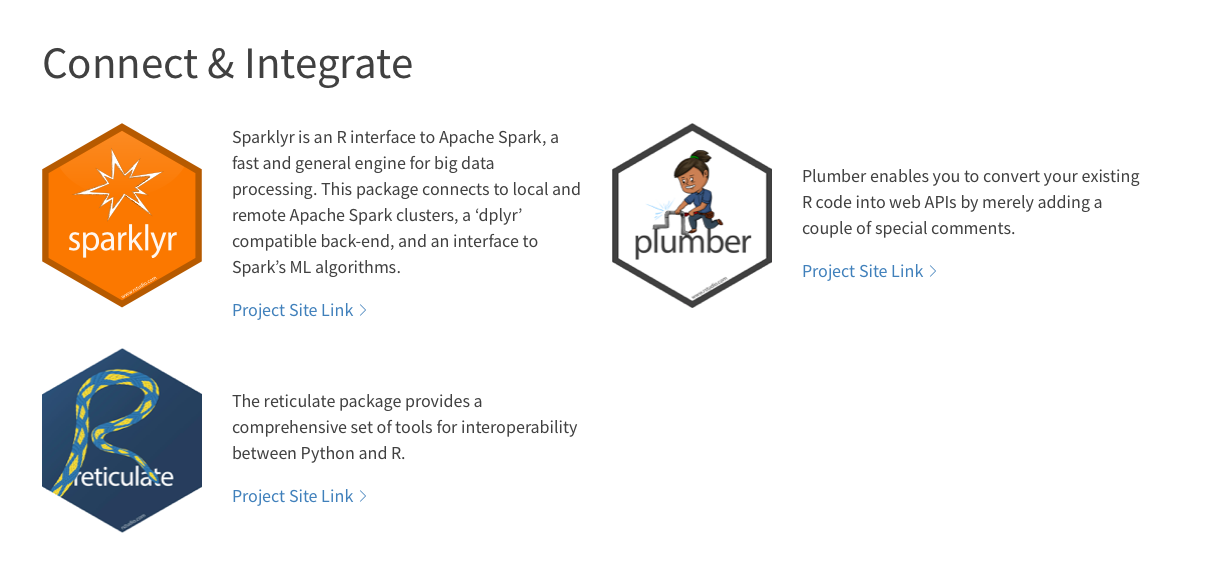
\includegraphics[width=0.85\textwidth,height=\textheight]{/Users/busenursarica/Desktop/R Lec Notes/comp3/_book/comp3_files/figure-html/P4.png}

\begin{center}\rule{0.5\linewidth}{0.5pt}\end{center}

\hypertarget{yuxfckleme-ve-tanux131ux15fma}{%
\chapter{Yükleme ve Tanışma}\label{yuxfckleme-ve-tanux131ux15fma}}

\hypertarget{yuxfckleme}{%
\section{Yükleme}\label{yuxfckleme}}

R'ın güncel versiyonun indirilmesi için \href{http://www.cran.r-project.org}{CRAN} (The Comprehensive R Archive Network) sayfası ziyaret edilmelidir. Bilgisayarınızdaki mevcut işletim sistemi için uygun olan versiyon indirilmelidir.

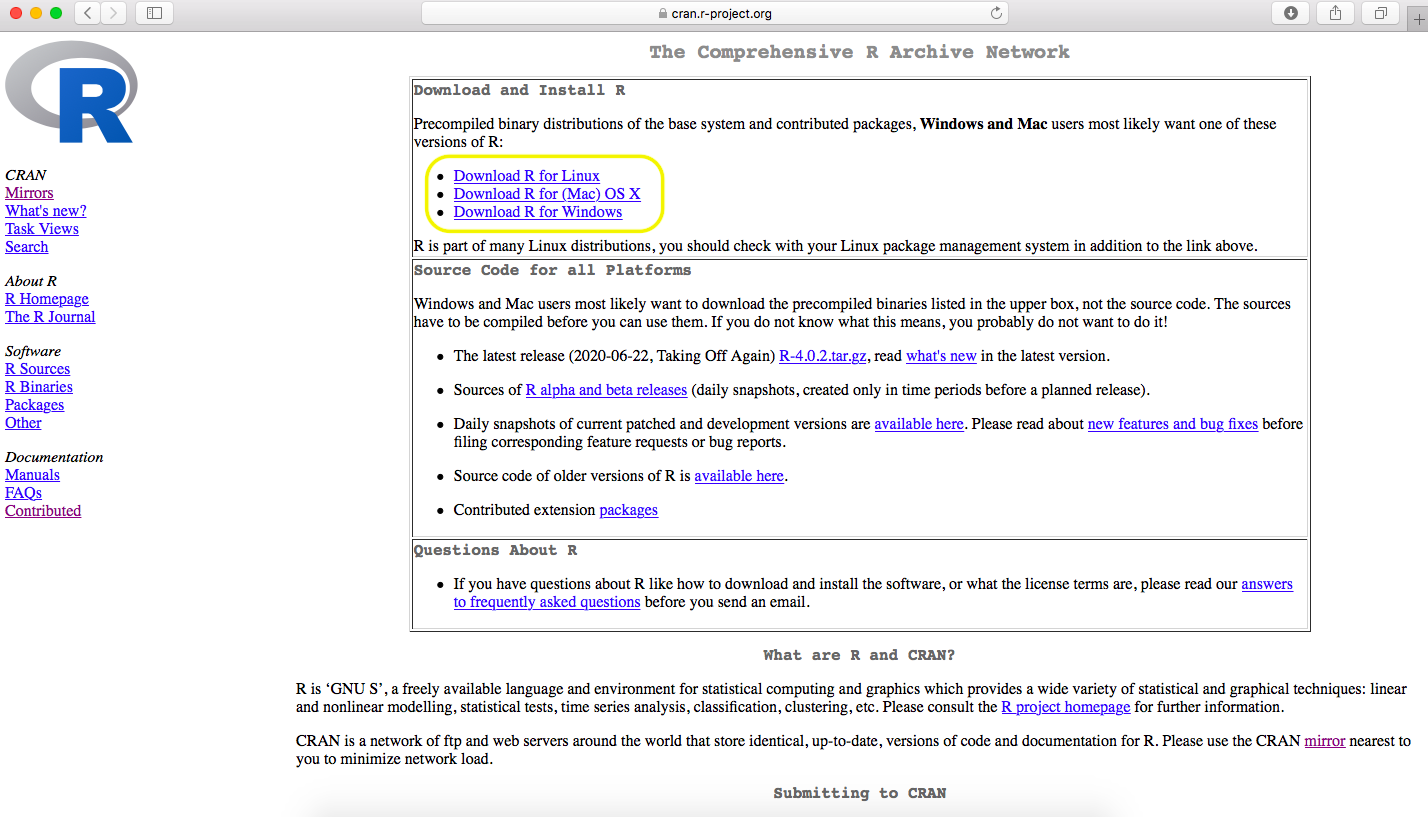
\includegraphics{/Users/busenursarica/Desktop/R Lec Notes/comp3/_book/comp3_files/figure-html/D1.png}

Uygun işletim sistemi seçildikten sonra \texttt{install\ R\ for\ the\ first\ time} tıklanarak temel versiyon seçilmelidir.

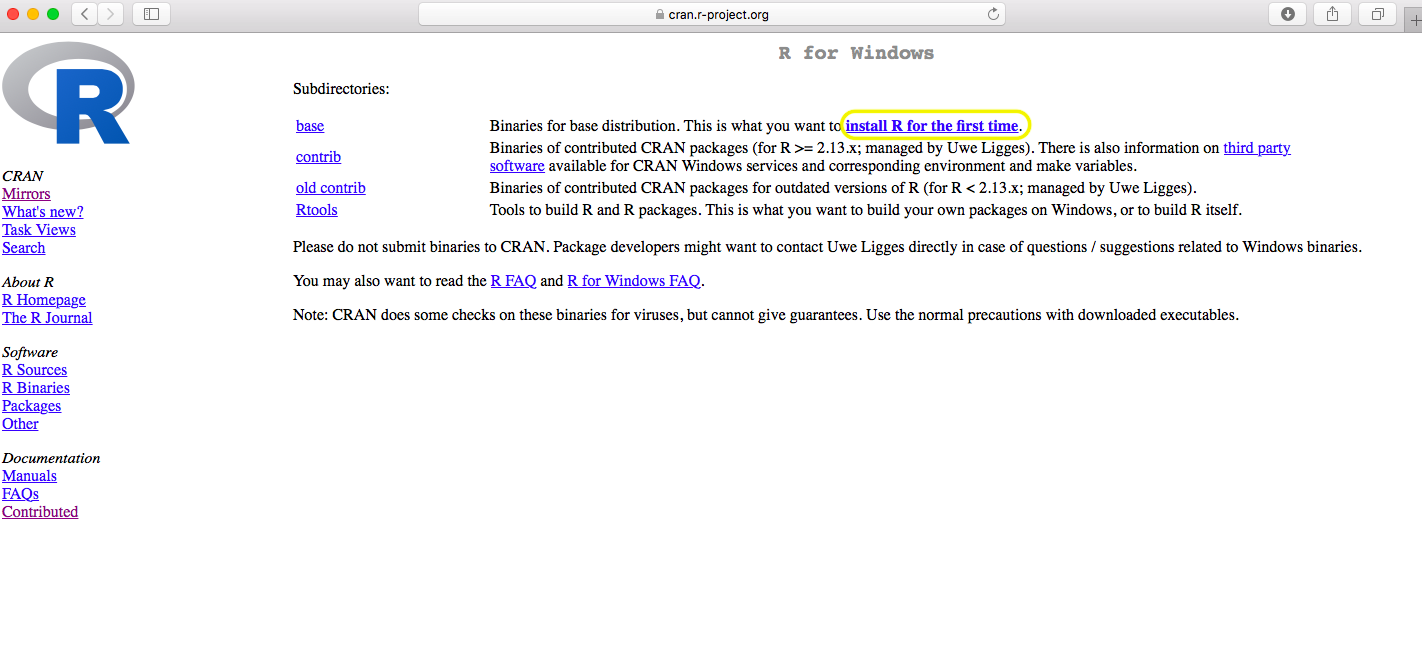
\includegraphics{/Users/busenursarica/Desktop/R Lec Notes/comp3/_book/comp3_files/figure-html/D2.png}

Gelen ekranda seçtiğiniz işletim sistemine uygun olan güncel R versiyonu görülecektir. \texttt{Download} işlemi başlatılır ve uygun seçenekler dahilinde indirme işlemi ve kurulum tamamlanır.

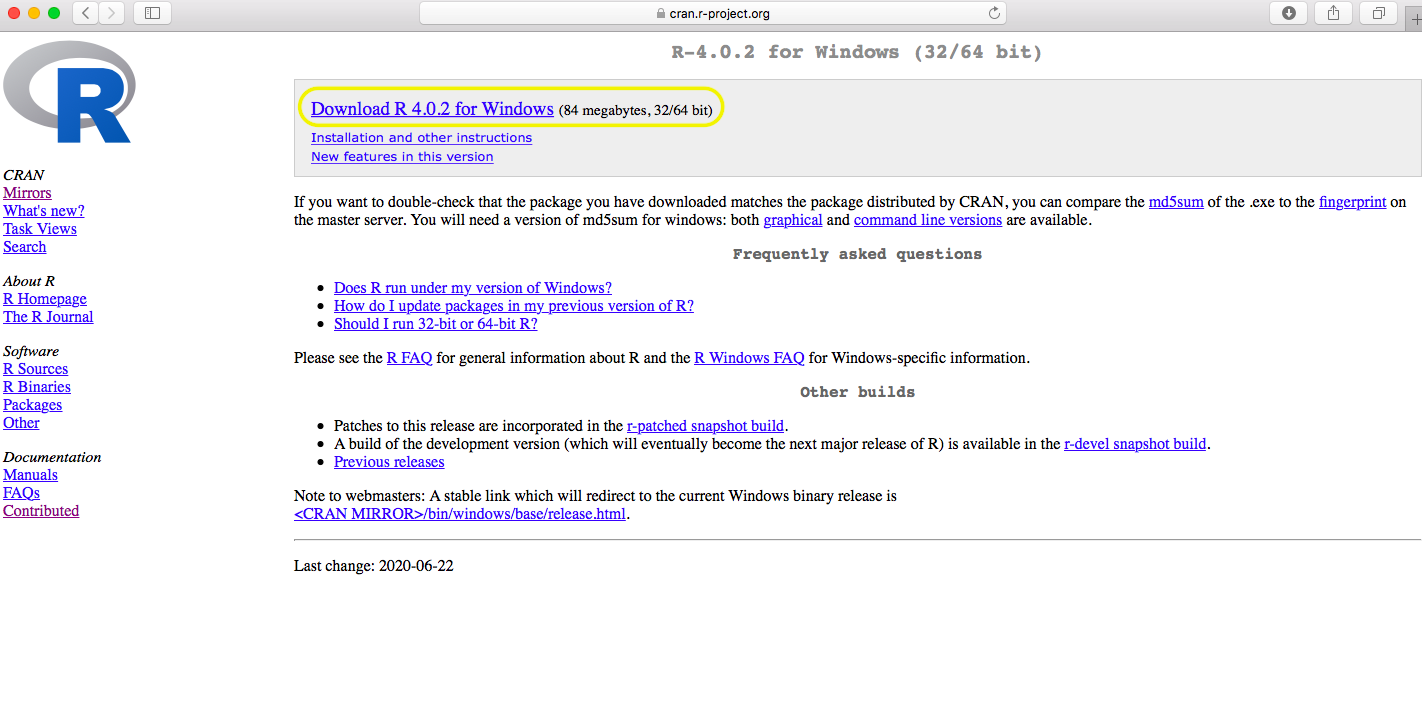
\includegraphics{/Users/busenursarica/Desktop/R Lec Notes/comp3/_book/comp3_files/figure-html/D3.png}

R yükleme işlemi tamamlandıktan sonra RStudio kurulum işlemine başlanır. \href{https://rstudio.com/products/rstudio/download/}{RStudio} sayfasına gidilir, bilgisayarınızdaki işletim sistemine uygun olan RStudio Desktop versiyonu indirilir ve kurulur.

\href{https://www.youtube.com/watch?v=Ohnk9hcxf9M\&feature=youtu.be}{Yükleme destek videosu (R-Windows)}

\href{https://www.youtube.com/watch?v=uxuuWXU-7UQ\&feature=youtu.be}{Yükleme destek videosu (R-Mac)}

\href{https://www.youtube.com/watch?v=bM7Sfz-LADM\&feature=youtu.be}{Yükleme destek videosu (RStudio)}

\begin{center}\rule{0.5\linewidth}{0.5pt}\end{center}

\hypertarget{tanux131ux15fma}{%
\section{Tanışma}\label{tanux131ux15fma}}

R programlama dilini kullanmak için console erişimi yeterlidir. Console yalın haliyle kullanılabildiği gibi RStudio aracılığı ile de kullanılabilir.

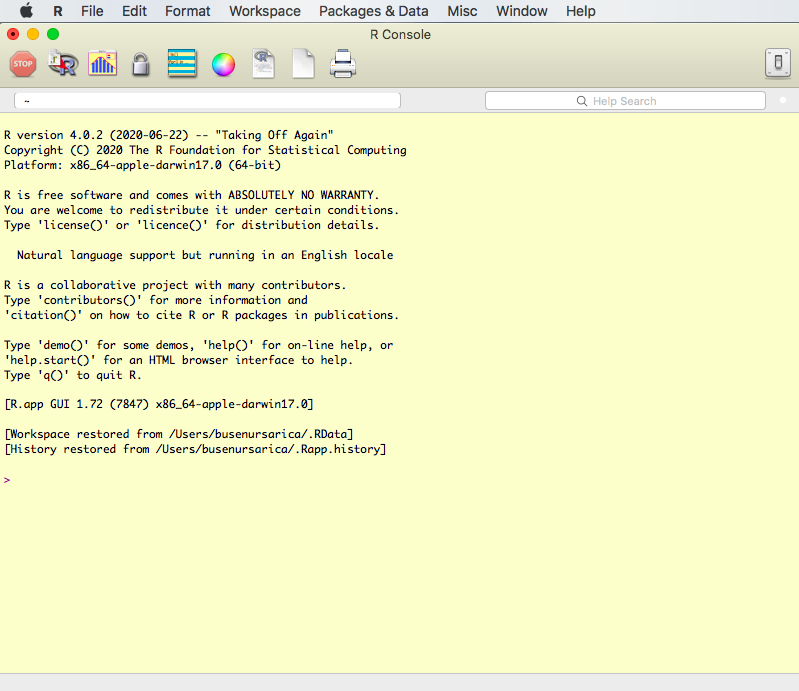
\includegraphics[width=0.7\textwidth,height=\textheight]{/Users/busenursarica/Desktop/R Lec Notes/comp3/_book/comp3_files/figure-html/00.png}

RStudio editor, görsel ve uygulama avantajları sayesinde uygulama kolaylığı sağlamaktadır.

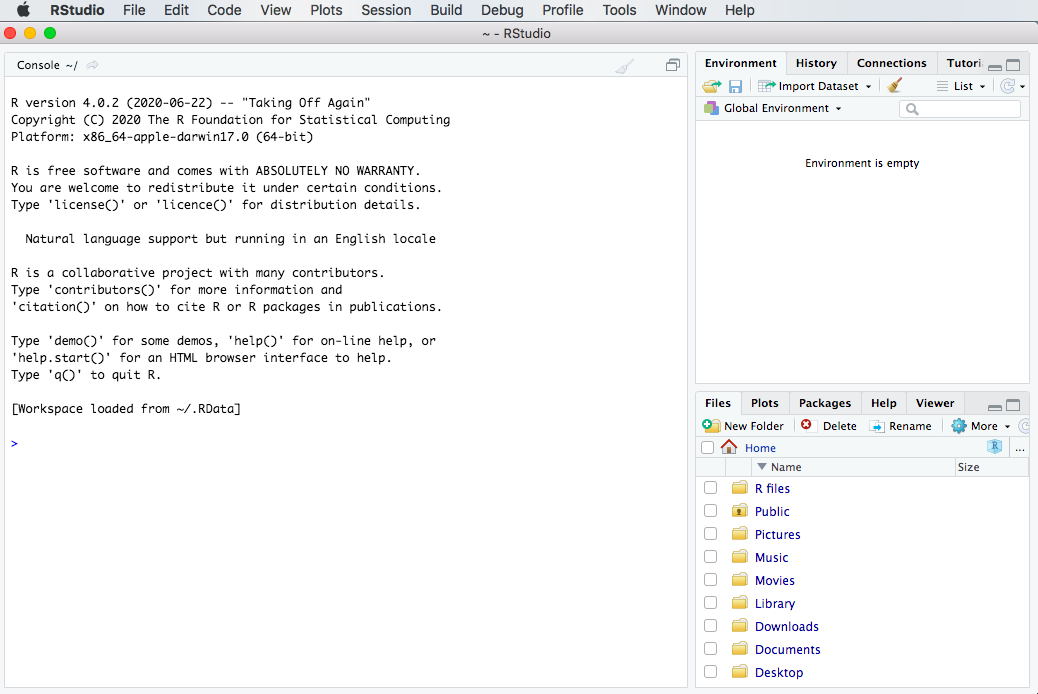
\includegraphics{/Users/busenursarica/Desktop/R Lec Notes/comp3/_book/comp3_files/figure-html/01.png}

R kullanarak yaptığınız çalışmalarda lütfen referans vermeyi unutmayınız.

\begin{Shaded}
\begin{Highlighting}[]
\KeywordTok{citation}\NormalTok{()}
\end{Highlighting}
\end{Shaded}

\begin{verbatim}
## 
## To cite R in publications use:
## 
##   R Core Team (2020). R: A language and environment for statistical
##   computing. R Foundation for Statistical Computing, Vienna, Austria.
##   URL https://www.R-project.org/.
## 
## A BibTeX entry for LaTeX users is
## 
##   @Manual{,
##     title = {R: A Language and Environment for Statistical Computing},
##     author = {{R Core Team}},
##     organization = {R Foundation for Statistical Computing},
##     address = {Vienna, Austria},
##     year = {2020},
##     url = {https://www.R-project.org/},
##   }
## 
## We have invested a lot of time and effort in creating R, please cite it
## when using it for data analysis. See also 'citation("pkgname")' for
## citing R packages.
\end{verbatim}

Yeni script oluşturmak için;

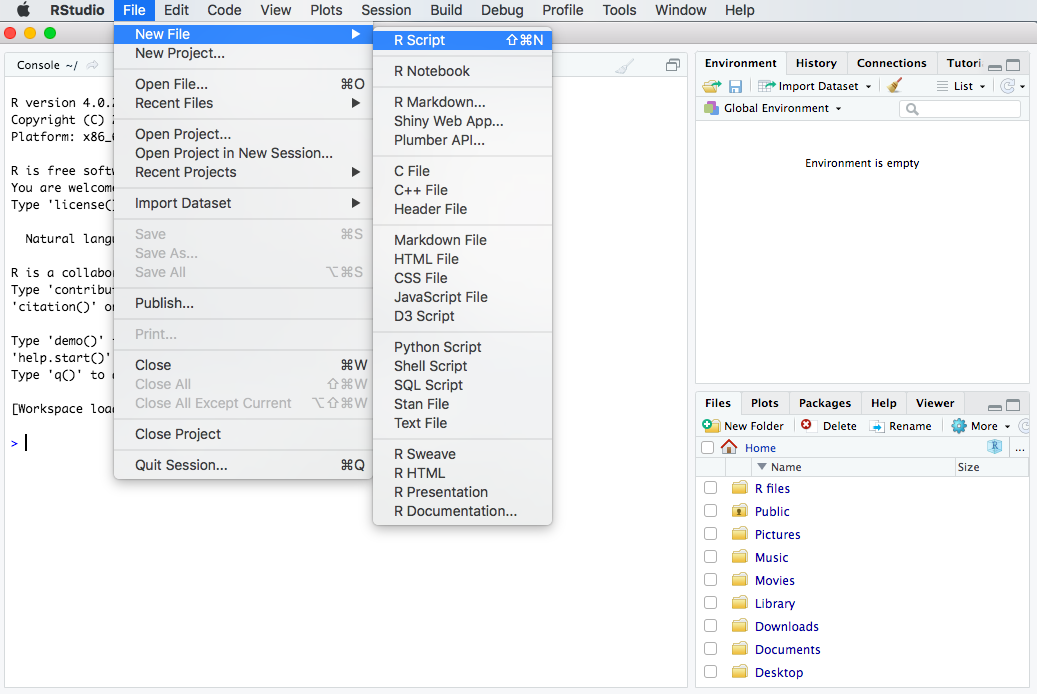
\includegraphics{/Users/busenursarica/Desktop/R Lec Notes/comp3/_book/comp3_files/figure-html/02.png}

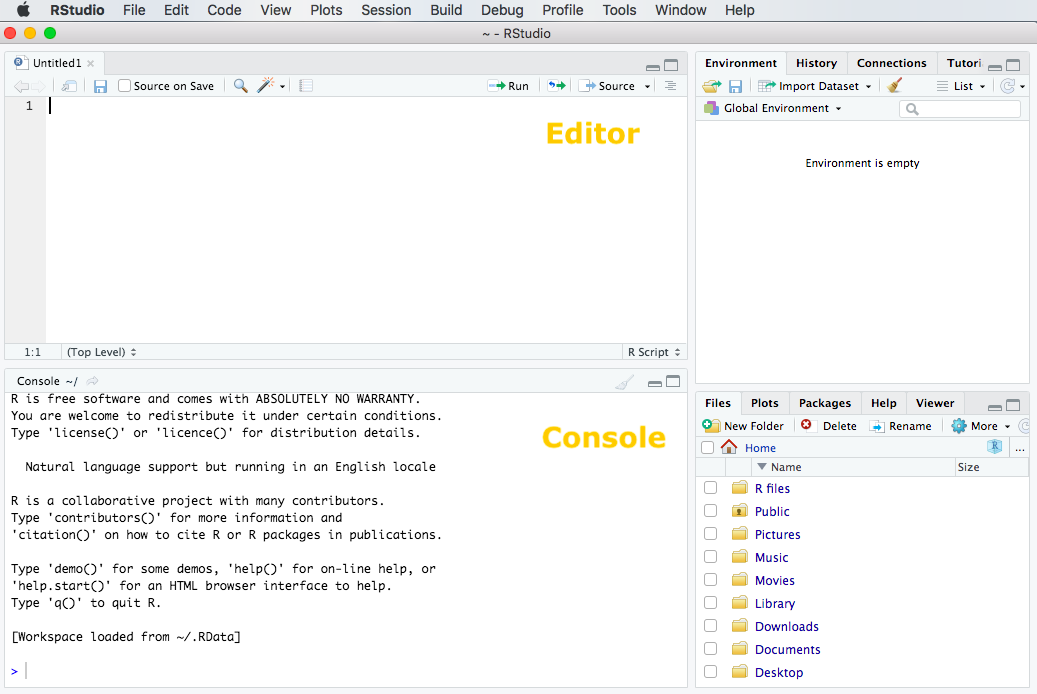
\includegraphics{/Users/busenursarica/Desktop/R Lec Notes/comp3/_book/comp3_files/figure-html/03.png}

RStudio cheatsheat yapısı sayesinde bir çok konu başlığında özet bilgiye ulaşmak mümkün.

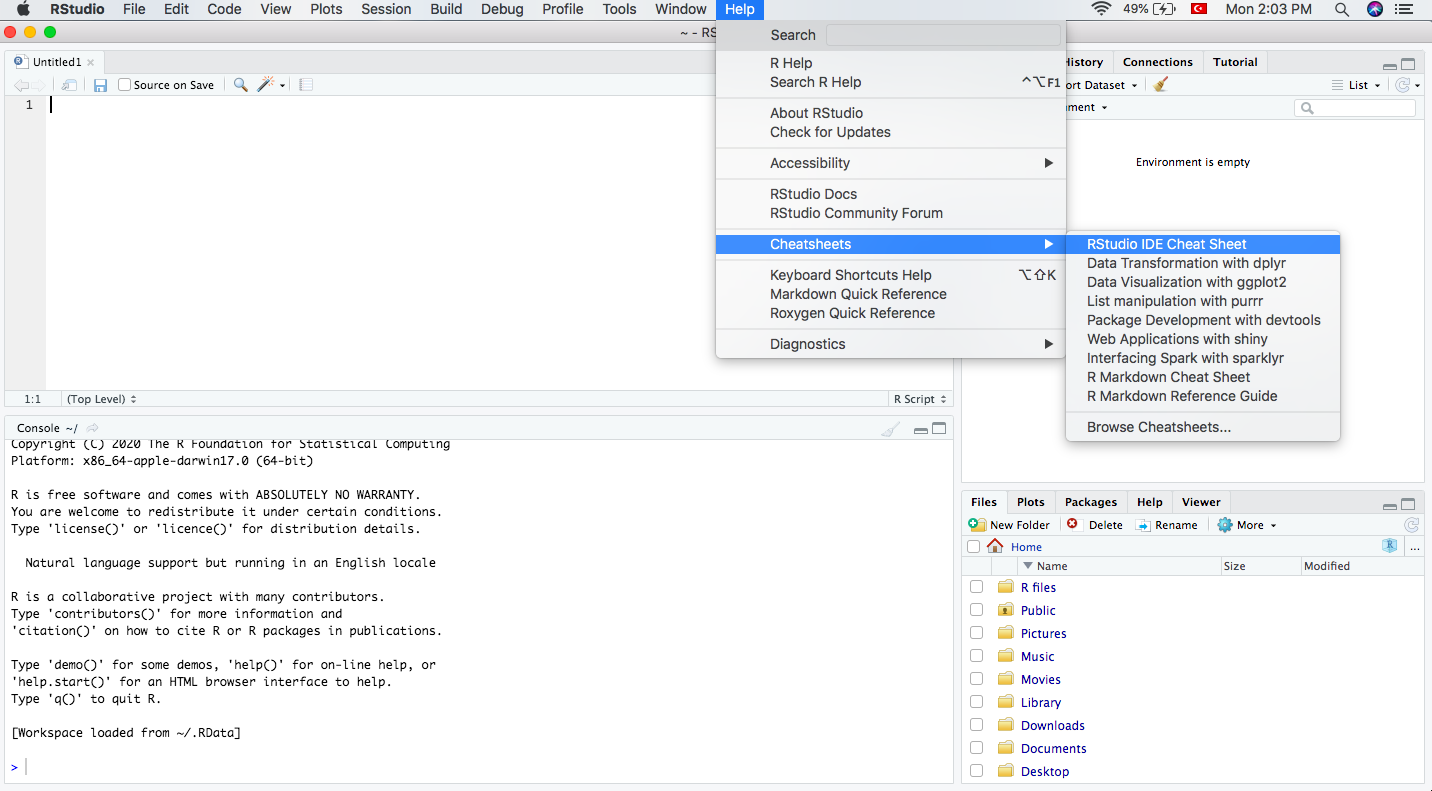
\includegraphics{/Users/busenursarica/Desktop/R Lec Notes/comp3/_book/comp3_files/figure-html/04.png}

\begin{center}\rule{0.5\linewidth}{0.5pt}\end{center}

\hypertarget{temel-nesneler}{%
\chapter{Temel Nesneler}\label{temel-nesneler}}

Bu bölümde kodlama için ihtiyaç duyacağınız temel yapılar açıklanacak ve uygulamalar ile desteklenecektir. \textbf{Farklı uygulamalar ders esnasında eş zamanlı yapılacağından lütfen online dersleri takip ediniz.}

\hypertarget{aritmetik-arithmetic}{%
\section{Aritmetik (Arithmetic)}\label{aritmetik-arithmetic}}

R, en basit haliyle hesap makinesi olarak kullanılabilir. Toplama \texttt{+}, çıkarma \texttt{-}, çarpma \texttt{*}, bölme \texttt{/} operatörleri ile gerçekleştirilir.

\begin{Shaded}
\begin{Highlighting}[]
\DecValTok{5}\OperatorTok{+}\DecValTok{4}
\end{Highlighting}
\end{Shaded}

\begin{verbatim}
## [1] 9
\end{verbatim}

Birden fazla matematiksel işlem aynı satırda gerçekleştirilebilir.

\begin{Shaded}
\begin{Highlighting}[]
\DecValTok{3}\OperatorTok{+}\DecValTok{4}\NormalTok{; }\DecValTok{6}\OperatorTok{*}\DecValTok{4}\NormalTok{; }\DecValTok{10-2}
\end{Highlighting}
\end{Shaded}

\begin{verbatim}
## [1] 7
\end{verbatim}

\begin{verbatim}
## [1] 24
\end{verbatim}

\begin{verbatim}
## [1] 8
\end{verbatim}

İşlemler parantez yardımıyla önceliğine göre yazılabilir, yazılmadığı taktirde matematiksel işlem önceliği geçerlidir.

\begin{Shaded}
\begin{Highlighting}[]
\DecValTok{10}\OperatorTok{*}\DecValTok{2-3}
\end{Highlighting}
\end{Shaded}

\begin{verbatim}
## [1] 17
\end{verbatim}

İşlem devam edecek biçimde tanımlanırsa console \texttt{+} simgesi ile devam edecek ve işlem tamamlanana kadar yeni işleme geçmenize engel olacaktır. İşlemi tamamlamalı veya yeni işleme geçmek için \texttt{esc} tuşunu kullanmalısınız.

\begin{Shaded}
\begin{Highlighting}[]
\DecValTok{10}\OperatorTok{+}\DecValTok{20}\OperatorTok{+}\DecValTok{30}\OperatorTok{+}
\StringTok{  }\DecValTok{40}
\end{Highlighting}
\end{Shaded}

\begin{verbatim}
## [1] 100
\end{verbatim}

Yapılan işlemler sonucu elde edilen çok büyük veya çok küçük sonuçlar için output exponent olarak verilir.

\begin{Shaded}
\begin{Highlighting}[]
\DecValTok{12000}\OperatorTok{*}\DecValTok{3000}
\end{Highlighting}
\end{Shaded}

\begin{verbatim}
## [1] 3.6e+07
\end{verbatim}

\begin{quote}
1.3e2 (130 anlamına gelir. e2: ondalık noktasını iki basamak sağa taşı)
\end{quote}

\begin{quote}
1.4e-1 (0.14 anlamına gelir. e-1: ondalık noktasını bir basamak sola taşı)
\end{quote}

Uygulamada elde edilen sonucun integer (tamsayı) olması gerekebilir. Bu noktada elde edilen output üste, alta veya 0.5 üzeri ya da altı olma durumuna göre farklı komutlar yardımı ile yuvarlanabilir.

\begin{itemize}
\tightlist
\item
  \textbf{floor:} alta yuvarla
\end{itemize}

\begin{Shaded}
\begin{Highlighting}[]
\KeywordTok{floor}\NormalTok{(}\FloatTok{5.2}\NormalTok{); }\KeywordTok{floor}\NormalTok{(}\FloatTok{5.7}\NormalTok{)}
\end{Highlighting}
\end{Shaded}

\begin{verbatim}
## [1] 5
\end{verbatim}

\begin{verbatim}
## [1] 5
\end{verbatim}

\begin{itemize}
\tightlist
\item
  \textbf{ceilign:} üste yuvarla
\end{itemize}

\begin{Shaded}
\begin{Highlighting}[]
\KeywordTok{ceiling}\NormalTok{(}\FloatTok{3.2}\NormalTok{); }\KeywordTok{ceiling}\NormalTok{(}\FloatTok{3.8}\NormalTok{)}
\end{Highlighting}
\end{Shaded}

\begin{verbatim}
## [1] 4
\end{verbatim}

\begin{verbatim}
## [1] 4
\end{verbatim}

\begin{itemize}
\tightlist
\item
  \textbf{round:} 0.5 üzeri ise üste, 0.5 altı ise alta yuvarla
\end{itemize}

\begin{Shaded}
\begin{Highlighting}[]
\KeywordTok{round}\NormalTok{(}\FloatTok{5.6}\NormalTok{); }\KeywordTok{round}\NormalTok{(}\FloatTok{5.3}\NormalTok{)}
\end{Highlighting}
\end{Shaded}

\begin{verbatim}
## [1] 6
\end{verbatim}

\begin{verbatim}
## [1] 5
\end{verbatim}

{Negatif sayılarda komutların nasıl işlediğini inceleyebilirsiniz. }

\textbf{round} komutu ile virgülden sonra kaç basamak olması gerektiğini belirterek yuvarlama işlemi yapabilirsiniz.

\begin{Shaded}
\begin{Highlighting}[]
\KeywordTok{round}\NormalTok{(}\FloatTok{1.248}\NormalTok{,}\DecValTok{2}\NormalTok{)}
\end{Highlighting}
\end{Shaded}

\begin{verbatim}
## [1] 1.25
\end{verbatim}

Kullanılabilecek matematiksel fonksiyonlara örnek olarak \citep{Crawley2012}

\begin{center}\rule{0.5\linewidth}{0.5pt}\end{center}

\hypertarget{nesneleri-tanux131mlama-assigning-objects}{%
\section{Nesneleri Tanımlama (Assigning Objects)}\label{nesneleri-tanux131mlama-assigning-objects}}

Temel işlevlerden bir diğeri kullanılacak değişkenlerin tanımlanmasıdır. Değişken için seçilecek isim mümkün olan en kısa haliyle tanımlanarak kavram kargaşası önlenmelidir.

\begin{itemize}
\item
  R, büyük ve küçük harfe duyarlıdır, dolayısıyla tanımlanan \(B\) ve \(b\) iki farklı değişkeni temsil eder.
\item
  Değişken ismi iki veya daha fazla kelimeden oluşacaksa kelimeler arasında boşluk yerine nokta kullanılmalıdır. (\sout{neura link})
\item
  Değişken ismi sayı veya sembol ile başlayamaz. (\sout{1a}, \sout{\&b})
\end{itemize}

Değişken tanımlama işlemi \texttt{\textless{}-} operatörü ile gerçekleştirilir. Tanımlanan değişken adı ile çağrılmazsa veya \texttt{print} komutu kullanılmazsa çıktı yazdırılmaz.

\begin{Shaded}
\begin{Highlighting}[]
\NormalTok{x<-}\DecValTok{3}
\KeywordTok{print}\NormalTok{(x)}
\end{Highlighting}
\end{Shaded}

\begin{verbatim}
## [1] 3
\end{verbatim}

Sayısal olmayan değer tanımlamaları tırnak içerisinde yapılmalıdır.

\begin{Shaded}
\begin{Highlighting}[]
\NormalTok{msg<-}\StringTok{ "hello world"}
\end{Highlighting}
\end{Shaded}

Tanımlanan değişken veya fonksiyon ile ilgili notlar \texttt{\#} ile tanımlanır.

\begin{Shaded}
\begin{Highlighting}[]
\NormalTok{x.ort<-}\DecValTok{20}  \CommentTok{# ortalama değer}
\end{Highlighting}
\end{Shaded}

Çıktıda basılan \texttt{{[}.{]}} kaçıncı gözlemden devam edildiğini gösterir. Örneğin 30 gözleminin \texttt{{[}26{]}} ifadesinin yardımı ile 26. gözlem olduğunu kolaylıkla söyleyebiliriz. \texttt{{[}.{]}} ifadeleri asıl seride yer almaz, yalnızca yol gösterici olarak çıktıda gözlenir.

\begin{Shaded}
\begin{Highlighting}[]
\NormalTok{x<-}\DecValTok{5}\OperatorTok{:}\DecValTok{50}
\NormalTok{x}
\end{Highlighting}
\end{Shaded}

\begin{verbatim}
##  [1]  5  6  7  8  9 10 11 12 13 14 15 16 17 18 19 20 21 22 23 24 25 26 27 28 29
## [26] 30 31 32 33 34 35 36 37 38 39 40 41 42 43 44 45 46 47 48 49 50
\end{verbatim}

\begin{center}\rule{0.5\linewidth}{0.5pt}\end{center}

\hypertarget{vektuxf6rler-vectors}{%
\section{Vektörler (Vectors)}\label{vektuxf6rler-vectors}}

Vektör oluşturmak için \texttt{c()} operatör kullanılmaktadır. Vektörler

\begin{itemize}
\tightlist
\item
  numeric
\item
  character
\item
  logical
\item
  integer
\item
  complex
\end{itemize}

yapıları içerebilir. \textbf{Vektörler yalnızca aynı yapıda gözlemler içerebilir.}

\begin{Shaded}
\begin{Highlighting}[]
\NormalTok{x <-}\StringTok{ }\KeywordTok{c}\NormalTok{(}\FloatTok{0.5}\NormalTok{, }\FloatTok{0.6}\NormalTok{) }\CommentTok{# numeric }
\NormalTok{x <-}\StringTok{ }\KeywordTok{c}\NormalTok{(}\OtherTok{TRUE}\NormalTok{, }\OtherTok{FALSE}\NormalTok{) }\CommentTok{# logical}
\NormalTok{x <-}\StringTok{ }\KeywordTok{c}\NormalTok{(T, F) }\CommentTok{# logical}
\NormalTok{x <-}\StringTok{ }\KeywordTok{c}\NormalTok{(}\StringTok{"a"}\NormalTok{, }\StringTok{"b"}\NormalTok{, }\StringTok{"c"}\NormalTok{) }\CommentTok{# character}
\NormalTok{x <-}\StringTok{ }\DecValTok{9}\OperatorTok{:}\DecValTok{29} \CommentTok{# integer}
\NormalTok{x <-}\StringTok{ }\KeywordTok{c}\NormalTok{(}\DecValTok{1}\OperatorTok{+}\NormalTok{0i, }\DecValTok{2}\OperatorTok{+}\NormalTok{4i) }\CommentTok{# complex}
\end{Highlighting}
\end{Shaded}

\texttt{T} ve \texttt{F}, \texttt{TRUE} ve \texttt{FALSE}'a karşılık kullanılan kısaltma yapılardır.

\begin{Shaded}
\begin{Highlighting}[]
\NormalTok{x <-}\StringTok{ }\KeywordTok{c}\NormalTok{(T, F) }\CommentTok{# logical}
\NormalTok{x}
\end{Highlighting}
\end{Shaded}

\begin{verbatim}
## [1]  TRUE FALSE
\end{verbatim}

Aynı zamanda \texttt{vector} komutu ile de vektör oluşturabilirsiniz. Vektörü tanımlarken belirlenen içerik yapısına göre oluşturulur.

\begin{Shaded}
\begin{Highlighting}[]
\NormalTok{x <-}\StringTok{ }\KeywordTok{vector}\NormalTok{(}\StringTok{"numeric"}\NormalTok{, }\DataTypeTok{length =} \DecValTok{7}\NormalTok{)}
\NormalTok{x}
\end{Highlighting}
\end{Shaded}

\begin{verbatim}
## [1] 0 0 0 0 0 0 0
\end{verbatim}

Karakter elemanları içerecek bir vektör oluşturmak istendiğinde;

\begin{Shaded}
\begin{Highlighting}[]
\NormalTok{x <-}\StringTok{ }\KeywordTok{vector}\NormalTok{(}\StringTok{"complex"}\NormalTok{, }\DataTypeTok{length =} \DecValTok{7}\NormalTok{)}
\NormalTok{x}
\end{Highlighting}
\end{Shaded}

\begin{verbatim}
## [1] 0+0i 0+0i 0+0i 0+0i 0+0i 0+0i 0+0i
\end{verbatim}

\begin{quote}
Aynı değişken adı birden fazla tanımlamada kullanılırsa yapılan son tanımlama geçerli olacaktır. Kod yazarken kullandığınız değişken isimlerine ve doğru yazıma dikkat ediniz.
\end{quote}

\textbf{Vektör aynı yapıda gözlemlerden oluşmuyorsa?}

Bu durumda tüm gözlemler tek bir yapı olarak algılanır. Herhangi bir değişkenin hangi yapıda gözlem içerdiği \texttt{class()} komutu ile sorgulanabilir.

\begin{Shaded}
\begin{Highlighting}[]
\NormalTok{y <-}\StringTok{ }\KeywordTok{c}\NormalTok{(}\FloatTok{1.7}\NormalTok{, }\StringTok{"a"}\NormalTok{)  }\CommentTok{# character }
\KeywordTok{class}\NormalTok{(y)}
\end{Highlighting}
\end{Shaded}

\begin{verbatim}
## [1] "character"
\end{verbatim}

\begin{Shaded}
\begin{Highlighting}[]
\NormalTok{y <-}\StringTok{ }\KeywordTok{c}\NormalTok{(}\OtherTok{TRUE}\NormalTok{, }\DecValTok{2}\NormalTok{) }\CommentTok{# numeric}
\KeywordTok{class}\NormalTok{(y)}
\end{Highlighting}
\end{Shaded}

\begin{verbatim}
## [1] "numeric"
\end{verbatim}

\begin{Shaded}
\begin{Highlighting}[]
\NormalTok{y <-}\StringTok{ }\KeywordTok{c}\NormalTok{(}\StringTok{"a"}\NormalTok{, }\OtherTok{TRUE}\NormalTok{) }\CommentTok{# character}
\KeywordTok{class}\NormalTok{(y)}
\end{Highlighting}
\end{Shaded}

\begin{verbatim}
## [1] "character"
\end{verbatim}

\begin{quote}
Vektör farklı yapıda gözlemler için verimli kullanılamıyor olabilir ancak bu işlemi gerçekleştirebilen \texttt{list} komutu mevcuttur. İlerleyen başlıklarda bu komut detaylandırılacaktır.
\end{quote}

Kodlama yaparken sıklıkla kullanılan bir işlem türü de vektör yapısının değiştirilmesidir. Vektör içeriğinin aynı yapıda olması kuralına sadık kalarak tüm vektör içeriği farklı bir yapıya aktarılabilir. Burada \texttt{as.numeric}, \texttt{as.logical} gibi komutlardan faydalanılır.

\begin{Shaded}
\begin{Highlighting}[]
\NormalTok{x <-}\StringTok{ }\DecValTok{0}\OperatorTok{:}\DecValTok{6}
\KeywordTok{class}\NormalTok{(x)}
\end{Highlighting}
\end{Shaded}

\begin{verbatim}
## [1] "integer"
\end{verbatim}

x vektörünün \texttt{integer} yapıda olduğunu gördükten sonra \texttt{as.character} komutu ile yeni x vektörünü \texttt{numeric} olarak tanımlayabiliriz.

\begin{Shaded}
\begin{Highlighting}[]
\NormalTok{x<-}\KeywordTok{as.character}\NormalTok{(x)}
\NormalTok{x; }\KeywordTok{class}\NormalTok{(x)}
\end{Highlighting}
\end{Shaded}

\begin{verbatim}
## [1] "0" "1" "2" "3" "4" "5" "6"
\end{verbatim}

\begin{verbatim}
## [1] "character"
\end{verbatim}

Bazı durumlarda R dönüşüm için çözüm üretemez ve \texttt{NA} çıktı verir.

\begin{Shaded}
\begin{Highlighting}[]
\NormalTok{x <-}\StringTok{ }\KeywordTok{c}\NormalTok{(}\StringTok{"a"}\NormalTok{, }\StringTok{"b"}\NormalTok{, }\StringTok{"c"}\NormalTok{)}
\KeywordTok{as.numeric}\NormalTok{(x)}
\end{Highlighting}
\end{Shaded}

\begin{verbatim}
## Warning: NAs introduced by coercion
\end{verbatim}

\begin{verbatim}
## [1] NA NA NA
\end{verbatim}

\begin{center}\rule{0.5\linewidth}{0.5pt}\end{center}

\hypertarget{matrisler-matrices}{%
\section{Matrisler (Matrices)}\label{matrisler-matrices}}

Matrisler, boyut niteliğine sahip vektörlerdir. Matris yapısında \emph{satır (row)} ve \emph{sütun (column)} tanımlanması gündeme gelmektedir. m içeriği boş bir matris olmak üzere;

\begin{Shaded}
\begin{Highlighting}[]
\NormalTok{m <-}\StringTok{ }\KeywordTok{matrix}\NormalTok{(}\DataTypeTok{nrow =} \DecValTok{2}\NormalTok{, }\DataTypeTok{ncol =} \DecValTok{3}\NormalTok{)}
\NormalTok{m}
\end{Highlighting}
\end{Shaded}

\begin{verbatim}
##      [,1] [,2] [,3]
## [1,]   NA   NA   NA
## [2,]   NA   NA   NA
\end{verbatim}

Matris boyutu \texttt{dim()} komutu ile sorgulanır.

\begin{Shaded}
\begin{Highlighting}[]
\KeywordTok{dim}\NormalTok{(m)}
\end{Highlighting}
\end{Shaded}

\begin{verbatim}
## [1] 2 3
\end{verbatim}

Matris yapısında gözlemler sütun şeklinde sıralanır.

\begin{Shaded}
\begin{Highlighting}[]
\NormalTok{m <-}\StringTok{ }\KeywordTok{matrix}\NormalTok{(}\DecValTok{1}\OperatorTok{:}\DecValTok{6}\NormalTok{, }\DataTypeTok{nrow =} \DecValTok{2}\NormalTok{, }\DataTypeTok{ncol =} \DecValTok{3}\NormalTok{) }
\NormalTok{m}
\end{Highlighting}
\end{Shaded}

\begin{verbatim}
##      [,1] [,2] [,3]
## [1,]    1    3    5
## [2,]    2    4    6
\end{verbatim}

Vektörler parçalanarak da matris yapısı oluşturabilirler.

\begin{Shaded}
\begin{Highlighting}[]
\NormalTok{m <-}\StringTok{ }\DecValTok{1}\OperatorTok{:}\DecValTok{10}\NormalTok{ ;m}
\end{Highlighting}
\end{Shaded}

\begin{verbatim}
##  [1]  1  2  3  4  5  6  7  8  9 10
\end{verbatim}

\begin{Shaded}
\begin{Highlighting}[]
\KeywordTok{dim}\NormalTok{(m) <-}\StringTok{ }\KeywordTok{c}\NormalTok{(}\DecValTok{2}\NormalTok{, }\DecValTok{5}\NormalTok{) ;m}
\end{Highlighting}
\end{Shaded}

\begin{verbatim}
##      [,1] [,2] [,3] [,4] [,5]
## [1,]    1    3    5    7    9
## [2,]    2    4    6    8   10
\end{verbatim}

Matrisler, satır veya sütunların birleştirilmesi yoluyla da oluşturulabilir. Satıların bir araya getirilmesi için \texttt{rbind} komutu kullanılırken, sütunların bir araya getirilmesi için \texttt{cbind} komutu kullanılmaktadır.

\begin{Shaded}
\begin{Highlighting}[]
\NormalTok{x <-}\StringTok{ }\DecValTok{1}\OperatorTok{:}\DecValTok{3}
\NormalTok{y <-}\StringTok{ }\DecValTok{10}\OperatorTok{:}\DecValTok{12}
\KeywordTok{cbind}\NormalTok{(x, y)}
\end{Highlighting}
\end{Shaded}

\begin{verbatim}
##      x  y
## [1,] 1 10
## [2,] 2 11
## [3,] 3 12
\end{verbatim}

\begin{Shaded}
\begin{Highlighting}[]
\KeywordTok{rbind}\NormalTok{(x, y)}
\end{Highlighting}
\end{Shaded}

\begin{verbatim}
##   [,1] [,2] [,3]
## x    1    2    3
## y   10   11   12
\end{verbatim}

\begin{center}\rule{0.5\linewidth}{0.5pt}\end{center}

\hypertarget{listeler-ve-data-frameler-lists-and-data-frames}{%
\section{Listeler ve Data Frameler (Lists and Data Frames)}\label{listeler-ve-data-frameler-lists-and-data-frames}}

\begin{center}\rule{0.5\linewidth}{0.5pt}\end{center}

\hypertarget{nuxfcmerik-olmayan-deux11ferler-non-numeric-values}{%
\section{Nümerik Olmayan Değerler (Non-Numeric Values)}\label{nuxfcmerik-olmayan-deux11ferler-non-numeric-values}}

\begin{center}\rule{0.5\linewidth}{0.5pt}\end{center}

\hypertarget{mantux131k-iux15flemleri}{%
\subsection{Mantık İşlemleri}\label{mantux131k-iux15flemleri}}

\begin{center}\rule{0.5\linewidth}{0.5pt}\end{center}

\hypertarget{karakterler}{%
\subsection{Karakterler}\label{karakterler}}

\begin{center}\rule{0.5\linewidth}{0.5pt}\end{center}

\hypertarget{faktuxf6rler-factors}{%
\subsection{Faktörler (Factors)}\label{faktuxf6rler-factors}}

\begin{center}\rule{0.5\linewidth}{0.5pt}\end{center}

\hypertarget{eksik-guxf6zlemler-missing-values}{%
\section{Eksik Gözlemler (Missing Values)}\label{eksik-guxf6zlemler-missing-values}}

\hypertarget{import-export-iux15flemleri}{%
\chapter{Import Export İşlemleri}\label{import-export-iux15flemleri}}

\hypertarget{references}{%
\chapter{References}\label{references}}

\hypertarget{dplyr}{%
\chapter{DPLYR}\label{dplyr}}

\hypertarget{apply-ailesi}{%
\chapter{Apply Ailesi}\label{apply-ailesi}}

\hypertarget{grafikler}{%
\chapter{Grafikler}\label{grafikler}}

\hypertarget{duxf6nguxfcler}{%
\chapter{Döngüler}\label{duxf6nguxfcler}}

\hypertarget{fonksiyonlar}{%
\chapter{Fonksiyonlar}\label{fonksiyonlar}}

\hypertarget{referans}{%
\chapter{Referans}\label{referans}}

  \bibliography{book.bib,packages.bib}

\end{document}
